El precio PVPC (Precio Voluntario para el Pequeño Consumidor) para península se
obtiene desde el portal \textbf{ESIOS} de Red Eléctrica de España
\footnote{\url{https://www.esios.ree.es/es/analisis/1001?geoids=8741}}, donde
se encuentran disponibles para comparación y descarga multitud de datos.
Mientras que los precios de venta de excedentes del autoconsumo con
compensación simplificada son iguales a los precios de mercado diario que se
presentan en la página del OMIE (Operador del Mercado Ibérico de Energía)
\footnote{\url{https://www.omie.es/es/file-access-list}}.

Ambos se muestran en la figura \ref{fig:prices_year}.

\begin{figure}[h] \centering
	\centering
	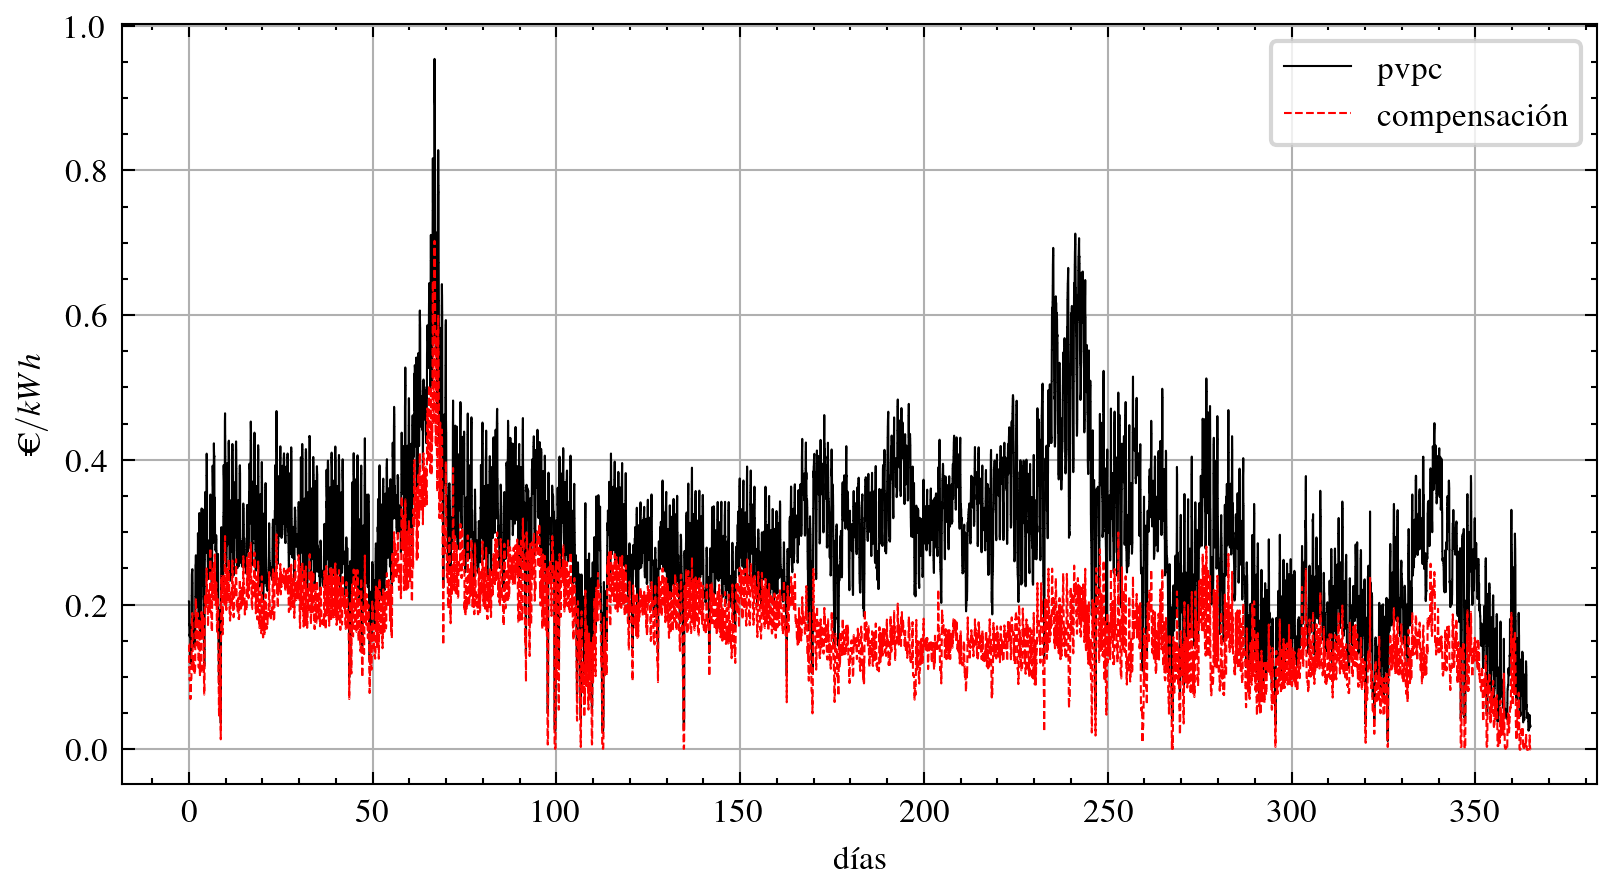
\includegraphics[width=1\textwidth]{./capitulos/adquisicion_de_datos/images/prices_year.png}
	\caption{Precios PVPC y diario en península para el año 2022.}
	\label{fig:prices_year}
\end{figure}
